\chapter{Lima Indra}\label{ch:g1:the-five-senses}

Pejamkan matamu dan dunia tidak lenyap: kamu masih mendengar suara
kelas, mencium bau masakan siang, merasakan kursi di bawahmu. Tubuh
mempunyai lima pintu menuju dunia --- indra --- dan tiap pintu adalah
sebuah alat tubuh yang bekerja untukmu sepanjang hari.

\section{Lima indra, lima alat}

\begin{definition}[Indra dan alat indra]\label{def:g1:the-five-senses:sense}
Suatu \emph{indra}\index{indra} adalah cara tubuh mencari tahu tentang
dunia. Tiap indra bekerja melalui sebuah \emph{alat
indra}\index{alat indra}, yaitu bagian tubuh yang dibangun untuk tugas
itu:
\begin{enumerate}
  \item \emph{penglihatan}\index{penglihatan} --- \emph{mata}\index{mata}
        melihat cahaya, warna dan bentuk;
  \item \emph{pendengaran}\index{pendengaran} --- \emph{telinga}\index{telinga}
        mendengar bunyi;
  \item \emph{penciuman}\index{penciuman} --- \emph{hidung}\index{hidung}
        mencium bau;
  \item \emph{pengecapan}\index{pengecapan} --- \emph{lidah}\index{lidah}
        mengecap makanan;
  \item \emph{perabaan}\index{perabaan} --- \emph{kulit}\index{kulit},
        di seluruh tubuh, merasakan kasar dan halus, hangat dan dingin.
\end{enumerate}
\end{definition}

\begin{example}[Sarapan, indra demi indra]\label{ex:g1:the-five-senses:breakfast}
Semangkuk cokelat panas memakai kelimanya: \omterm{def:g1:the-five-senses:sense}{mata} melihat uapnya, hidung
mencium bau kakaonya, \omterm{def:g1:the-five-senses:sense}{kulit} tangan merasakan mangkuk yang hangat,
\omterm{def:g1:the-five-senses:sense}{telinga} mendengar dentingan sendoknya, dan lidah --- bagian yang
terbaik --- mengecapnya.
\end{example}

\begin{omfigure}
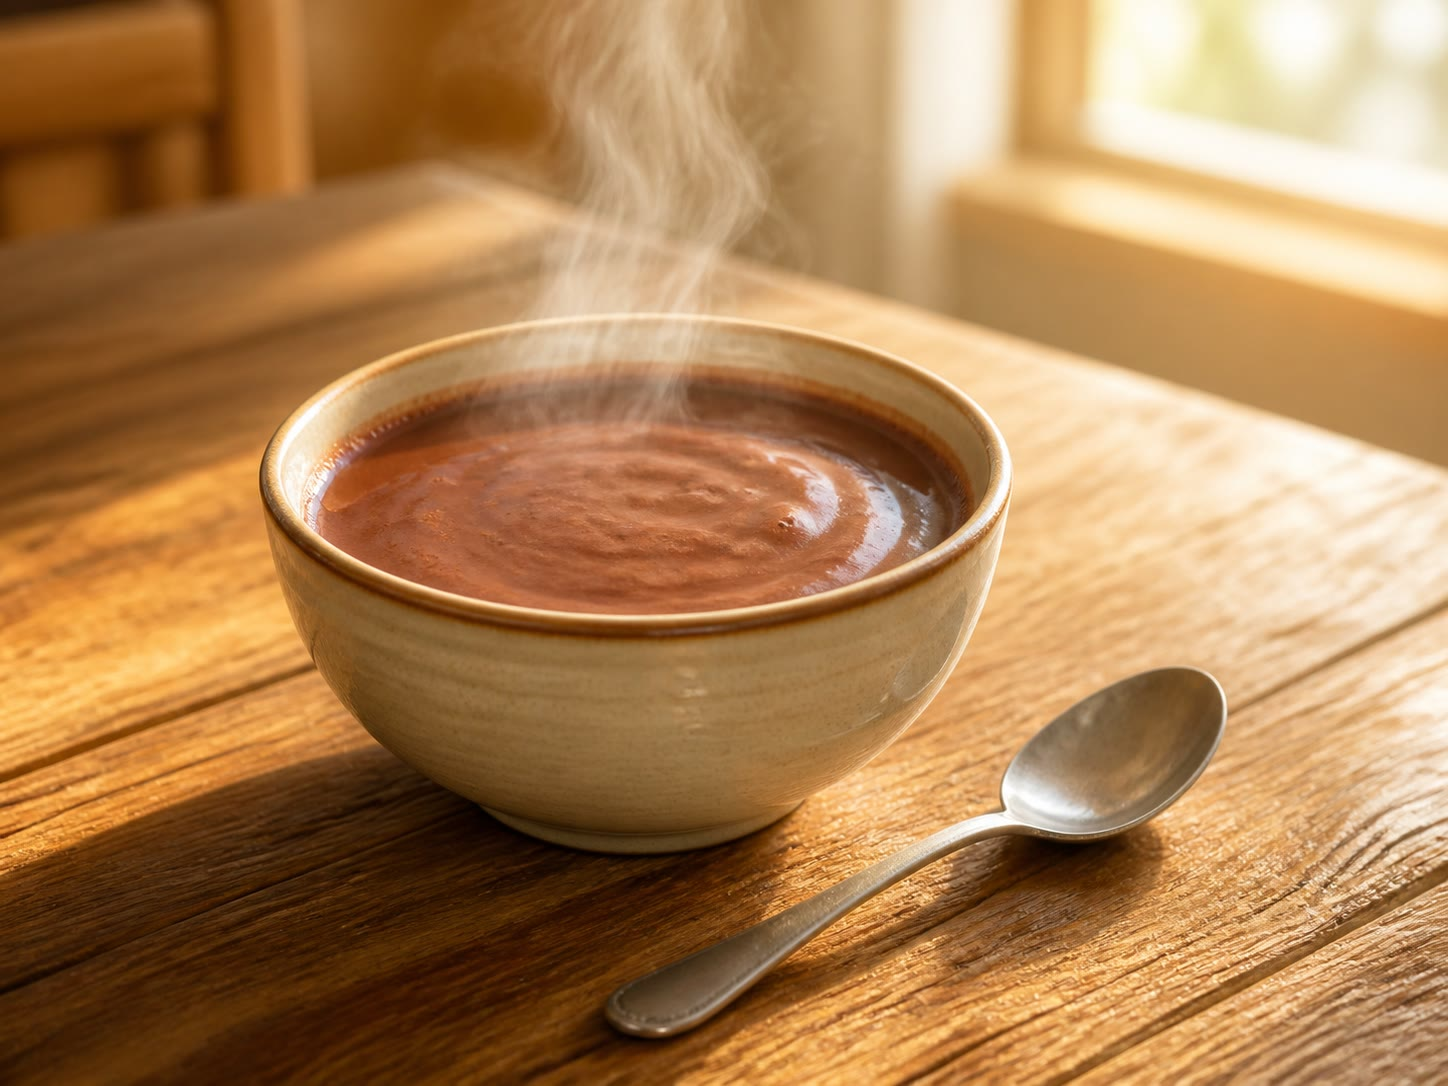
\includegraphics[width=0.58\linewidth]{images/book1/ai/g1-senses-chocolate.jpg}

{\small Semangkuk cokelat panas, lima indra bekerja sebelum tegukan
pertama.}
\end{omfigure}

\begin{remark}[Perabaan ada di mana-mana]\label{rem:g1:the-five-senses:skin}
Empat \omterm{def:g1:the-five-senses:sense}{alat indra} bertempat di kepala, tetapi alat perabaan adalah
\omterm{def:g1:the-five-senses:sense}{kulit}, dan \omterm{def:g1:the-five-senses:sense}{kulit} menyelimutimu dari ujung kepala sampai ujung kaki.
Itulah sebabnya kamu dapat merasakan embusan angin di lehermu,
sebutir kerikil di sepatumu dan seekor kepik yang hinggap di lenganmu
--- semuanya tanpa melihat.
\end{remark}

\section{Indra melapor kepada otak}

\begin{proposition}[Pesan kepada otak]\label{prop:g1:the-five-senses:brain}
Sebuah \omterm{def:g1:the-five-senses:sense}{alat indra} tidak memahami apa yang diinderanya --- ia
\emph{mengirim pesan}. Semua pesan itu menempuh perjalanan di dalam
tubuh menuju \emph{otak}\index{otak}, di dalam kepala, yang
merangkainya: ``itu suara Nenek'', ``bau itu roti panggang''. Tanpa
otak, \omterm{def:g1:the-five-senses:sense}{mata} dan \omterm{def:g1:the-five-senses:sense}{telinga} tak akan melapor kepada siapa pun.
\end{proposition}
\admitted

\begin{omfigure}
\begin{tikzpicture}[scale=0.9]
  % brain box
  \draw[thick, omDef, fill=omDef!8, rounded corners=6pt]
    (4.6,0.2) rectangle (8.2,2.0);
  \node[font=\small\bfseries, omDef] at (6.4,1.55) {otaknya};
  \node[font=\small, align=center, text width=3.2cm] at (6.4,0.85)
    {merangkai\\ pesan-pesannya};
  % organs
  \node[font=\small, left] (eye) at (2.2,2.6) {mata melihat};
  \node[font=\small, left] (ear) at (2.2,1.7) {telinga mendengar};
  \node[font=\small, left] (nose) at (2.2,0.8) {hidung mencium};
  \node[font=\small, left] (skin) at (2.2,-0.1) {kulit merasakan};
  % arrows
  \draw[->, thick, omMeth] (2.35,2.55) -- (4.55,1.75);
  \draw[->, thick, omMeth] (2.35,1.68) -- (4.55,1.35);
  \draw[->, thick, omMeth] (2.35,0.82) -- (4.55,0.95);
  \draw[->, thick, omMeth] (2.35,-0.02) -- (4.55,0.55);
  \node[font=\small, omMeth] at (3.4,3.0) {pesan};
\end{tikzpicture}

{\small Tiap \omterm{def:g1:the-five-senses:sense}{alat indra} mengirim pesannya kepada otak, yang memaknai
semuanya. (Lidah juga melapor --- gambarnya saja yang akan menjadi
terlalu penuh.)}
\end{omfigure}

\begin{example}[Menyebut benda dalam gelap]\label{ex:g1:the-five-senses:dark}
Seorang teman meletakkan benda yang sudah kamu kenal di tanganmu
ketika matamu terpejam: kunci, spons, sendok. Kamu menyebutnya hampir
seketika. \omterm{def:g1:the-five-senses:sense}{Kulit} mengirim pesannya --- dingin, keras, bergerigi --- dan
otak menjawab: ``sebuah kunci''. Indra mengumpulkan; otak memahami.
\end{example}

\begin{remark}[Saling menolong]\label{rem:g1:the-five-senses:together}
Indra bekerja sebagai satu regu. Makanan terasa ``hambar'' ketika
pilek menyumbat hidungmu, sebab penciuman mengerjakan separuh dari
cita rasanya. Dan ketika satu indra sama sekali tidak dapat
menjalankan tugasnya, indra yang lain belajar berbuat lebih banyak:
orang yang tidak dapat melihat membaca dengan ujung jarinya, memakai
perabaan, dan menyeberang jalan dengan \omterm{def:g1:the-five-senses:sense}{telinganya}.
\end{remark}

\section{Merawat alat indra}

\begin{proposition}[Pintu yang rapuh]\label{prop:g1:the-five-senses:fragile}
\omterm{def:g1:the-five-senses:sense}{Alat indra} sangat berharga dan mudah terluka. Bunyi yang terlalu keras
melukai \omterm{def:g1:the-five-senses:sense}{telinga}; memandang Matahari melukai \omterm{def:g1:the-five-senses:sense}{mata}; sesendok makanan
yang terlalu panas membakar lidah. \omterm{def:g1:the-five-senses:sense}{Alat indra} yang terluka mungkin
tetap terluka --- karena itu kita melindunginya.
\end{proposition}
\admitted

\begin{method}[Melindungi indraku]\label{met:g1:the-five-senses:protect}
\begin{enumerate}
  \item Jangan pernah memandang lurus ke Matahari, walau sekejap pun;
  \item jagalah bunyi tetap lembut: jangan berteriak ke \omterm{def:g1:the-five-senses:sense}{telinga}, pakai
        pengeras \omterm{def:g1:the-five-senses:sense}{telinga} pada suara pelan;
  \item jangan pernah memasukkan apa pun ke \omterm{def:g1:the-five-senses:sense}{telinga} atau hidungmu;
  \item tiuplah makanan panas sebelum mengecapnya;
  \item membaca dan menggambarlah dengan cahaya yang cukup.
\end{enumerate}
\end{method}

\begin{example}[Konser sebelah rumah]\label{ex:g1:the-five-senses:loud}
Sesudah musik yang sangat keras, \omterm{def:g1:the-five-senses:sense}{telinga} kadang berdenging beberapa
lama. Denging itu adalah \omterm{def:g1:the-five-senses:sense}{telinga} yang berkata ``terlalu banyak!''.
Orang yang bekerja dengan mesin yang berisik memakai penutup \omterm{def:g1:the-five-senses:sense}{telinga}
tepat karena alasan ini --- \omterm{def:g1:the-five-senses:sense}{telinga} mereka harus bertahan seumur
hidup.
\end{example}

\section{Latihan}

\begin{exercise}[$\star$]\label{exo:g1:the-five-senses:1}
Sebutkan kelima indra dan, untuk masing-masing, \omterm{def:g1:the-five-senses:sense}{alat indranya}.
\end{exercise}

\begin{exercise}[$\star$]\label{exo:g1:the-five-senses:2}
\omterm{def:g1:the-five-senses:sense}{Alat indra} mana yang melaporkan: (a) warna sebuah balon? (b) kelembutan
sebuah selimut? (c) bau hujan? (d) bunyi sebuah lonceng?
\end{exercise}

\begin{exercise}[$\star$]\label{exo:g1:the-five-senses:3}
\omterm{def:g1:the-five-senses:sense}{Alat indra} mana yang tidak berada di kepala? Sejauh mana jangkauannya?
\end{exercise}

\begin{exercise}[$\star$]\label{exo:g1:the-five-senses:4}
Pada \cref{ex:g1:the-five-senses:dark}, \omterm{def:g1:the-five-senses:sense}{matanya} terpejam. Alat mana
yang mengirim pesannya, dan bagian tubuh mana yang memahaminya?
\end{exercise}

\begin{exercise}[$\star$]\label{exo:g1:the-five-senses:5}
Ketika pilek dan hidung tersumbat, makanan seolah kehilangan cita
rasanya. Dua indra mana yang biasanya bekerja sama ketika kamu makan?
\end{exercise}

\begin{exercise}[$\star$]\label{exo:g1:the-five-senses:6}
Sebutkan tiga aturan \cref{met:g1:the-five-senses:protect}, dan
sebutkan \omterm{def:g1:the-five-senses:sense}{alat indra} mana yang dilindungi masing-masing.
\end{exercise}

\begin{exercise}[$\star$]\label{exo:g1:the-five-senses:7}
Mengapa orang yang bekerja dengan mesin yang berisik memakai penutup
\omterm{def:g1:the-five-senses:sense}{telinga}? Pakai \cref{prop:g1:the-five-senses:fragile}.
\end{exercise}

\begin{exercise}[$\star$]\label{exo:g1:the-five-senses:8}
Cobalah: dengan \omterm{def:g1:the-five-senses:sense}{mata} terpejam, mintalah seorang penolong menyodorkan
tiga jenis makanan di bawah hidungmu --- misalnya pisang, keju, jeruk.
Berapa banyak yang disebut hidungmu dengan benar, tanpa bantuan \omterm{def:g1:the-five-senses:sense}{mata}?
\end{exercise}

\begin{exercise}[$\star\star$]\label{exo:g1:the-five-senses:9}
Seorang teman mengaku: ``\omterm{def:g1:the-five-senses:sense}{Mata} memahami apa yang dilihatnya.''
Betulkan kalimat itu dengan \cref{prop:g1:the-five-senses:brain}: apa
yang sebenarnya dilakukan \omterm{def:g1:the-five-senses:sense}{mata}, dan siapa yang memahami?
\end{exercise}

\begin{exercise}[$\star\star$]\label{exo:g1:the-five-senses:10}
Bagaimana seseorang yang tidak dapat melihat dapat ``membaca'' buku,
dan menyeberang jalan dengan aman? Sebutkan indra mana yang mengambil
alih tugas yang mana.
\end{exercise}
